\documentclass[fleqn]{article}
\usepackage[spanish,es-noshorthands]{babel}
\usepackage[utf8]{inputenc} 
\usepackage[papersize={6.5in,8.5in},left=1cm, right=1cm, top=1.5cm, bottom=1.7cm]{geometry}
\usepackage{mathexam}
\usepackage{amsmath}
\usepackage{graphicx}
\usepackage{multicol}
\usepackage{tikz,pgf}

\ExamClass{
\includegraphics[height=16pt]{Images/logo-sed.png} Matemáticas $7^{\circ}$}
\ExamName{Números fraccionarios}
\ExamHead{
\includegraphics[height=16pt]{Images/logo-colegio.png} IEDAB}
\newcommand{\LineaNombre}{%
\par
\vspace{\baselineskip}
Nombre:\hrulefill \; Curso: \underline{\hspace*{48pt}} \; Fecha: \underline{\hspace*{2.5cm}} \relax
\par}
\let\ds\displaystyle

\begin{document}
\ExamInstrBox{
Respuesta sin justificar mediante procedimiento no será tenida en cuenta en la calificación. Escriba sus respuestas en el espacio indicado. Tiene 45 minutos para contestar esta prueba.}
\LineaNombre
\begin{enumerate}
 \item En las siguientes fracciones, distinga cuál es el numerador y cuál es el denominador y ubíquelas sobre la recta numérica.
 \begin{enumerate}
 \begin{multicols}{2}
 \item $\dfrac{3}{5}$
 \item $\dfrac{7}{5}$ 
 \end{multicols}
 \end{enumerate}
 \begin{tikzpicture}[scale=3]
\draw[<->] (-1,0)--(2.5,0);
\foreach \x in {0,1,2} \draw[shift={(\x,0)},color=black] (0pt,2pt) -- (0pt,-2pt) node[below] {\footnotesize $\x$};
\foreach \x in {-.8,-.6,-.4,-.2,0.2,.4,.6,.8,1.2,1.4,1.6,1.8,2.2,2.4} \draw[shift={(\x,0)},color=black] (0pt,1pt) -- (0pt,-1pt);
\end{tikzpicture}
 \item Determine la fracción correspondiente al área sombreada en cada dibujo.
 \begin{enumerate}
 \begin{multicols}{3}
 \item 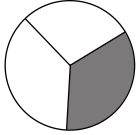
\includegraphics[scale=.4]{Images/Pantallazo-27.png} 
 \item 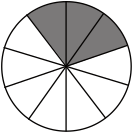
\includegraphics[scale=.4]{Images/Pantallazo-26.png} 
 \item  
\includegraphics[scale=.9]{Images/Pantallazo-2017-07-12-19-47-01.png} 
 \end{multicols}
 \end{enumerate}
 \item Para elaborar una torta se han utilizado 300 gr de harina, 200 gramos de zanahoria, 150 gr de mantequilla, 50 gr de azúcar y 100 gr de leche. ¿Qué fracción del total representan cada uno de estos ingredientes?\noanswer
 \newpage
 \item Calcule:
 \begin{enumerate}
 \item $\frac{3}{5}$ de 60 \noanswer
 \item $\frac{3}{8}$ de 48 \noanswer
 \item $\frac{7}{9}$ de 72 \noanswer
 \end{enumerate}
 \item Determine si cada una de las siguientes parejas de fracciones son equivalentes entre sí
 \begin{enumerate}
 \item $\dfrac{3}{5}$ y $\dfrac{21}{35}$ \noanswer
 \item $\dfrac{4}{7}$ y $\dfrac{36}{63}$ \noanswer
 \item $\dfrac{9}{11}$ y $\dfrac{18}{20}$ \noanswer
 \end{enumerate}
 \item Determine a qué fracción de \textbf{día} corresponden los siguientes números de horas. Simplifique la fracción a su mínima expresión.
 \begin{enumerate}
 \item 3 horas \noanswer
 \item 8 horas \noanswer
 \item 12 horas \noanswer
 \item 20 horas \noanswer
 \end{enumerate}
 \end{enumerate}

\end{document}
